\chapter{System Design\label{cha:design}}

As mentioned in Sec. \ref{sec:intro_strategy}, the overall target of this project is to develop four electronic modules and an electro-pneumatic actuation system for the 2010 Formula SAE vehicle. This chapter describes the design of these modules and the electro-pneumatic system, and provides context for design choices. The electrical portions of the design will be discussed in more detail than the mechanical portions, as the main focus of the thesis is electrical. 

Figure \ref{fig:design_overview} shows the electrical and mechanical interrelations between the 4 custom modules (in blue) and the systems they interact with. All of the modules communicate over a shared CAN bus network, which eliminates point-to-point wiring between them. The use of a CAN-based network was dictated by the use of the ECU, which uses a CAN interface to output data required by the modules. 

\begin{figure}[H]
\centering
\begin{tikzpicture}[auto, node distance=2cm, draw=black!70, >=stealth']
  \node [bus] (bus1) {};
  \node [bus, below of=bus1] (bus2) {};
  \node [bus, below of=bus2, label={[rotate=-90]below:CAN Bus}] (bus3) {};

  \draw [-, line width=3pt] ($(bus1)+(0,1cm)$) -- (bus1) -- (bus2) -- (bus3) -- ++(0,-1cm);

  \node [block, right of=bus2, minimum width=2cm] (ecu) {ECU};
  \node [block, right of=ecu, font=\scriptsize, node distance=3cm] (engine) {Engine};
  \draw [<->, thick] (ecu) -- (bus2);
  \draw [<->, thick, dashed] (engine) -- (ecu);

  \node [block, blue shiny, right of=bus1, text width=1.7cm] (telemetry_module) {Telemetry Module};
  \node [block, right of=telemetry_module, text width=1.5cm, node distance=3cm] (dac) {DAQ};
  \draw [<->, thick] (telemetry_module) -- (bus1);
  \draw [<-, thick] (telemetry_module) -- (dac);
  \draw [->, thick] (ecu) -- (telemetry_module);
  \draw [-, thick] (telemetry_module.north) \antenna;

  \node [block, blue shiny, left of=bus1, text width=1.5cm] (brake_module) {Brake Module};
  \node [block, left of=brake_module, font=\scriptsize, text width=1.5cm, node distance=3cm] (brakes) {Braking System};
  \draw [<->, thick] (brake_module) -- (bus1);
  \draw [<->, thick, dashed] (brake_module) -- (brakes);
  
  \node [block, blue shiny, left of=bus2, text width=1.6cm] (engine_module) {Eng. \& Trans. Module};
  \node [block, left of=engine_module, font=\scriptsize, node distance=3cm] (intake) {Intake};
  \node [block, below of=engine_module, text width=2cm] (pneumatics) {Electro-pneumatics};
  \node [block, left of=pneumatics, font=\scriptsize, node distance=3cm] (transmission) {Transmission};
  \draw [<->, thick] (engine_module) -- (bus2);
  \draw [<->, thick, dashed] (engine_module) -- (intake);
  \draw [->, thick] (engine_module) -- (pneumatics);
  \draw [<->, thick, dashed] (pneumatics) -- (transmission);
  \draw [->, thick] (transmission) -- (engine_module);

  \node [block, blue shiny, right of=bus3, text width=1.6cm] (driver_interface) {Driver Interface Module};
  \node [block, right of=driver_interface, node distance=3cm, text width=1.25cm, font=\scriptsize] (controls) {Steering wheel controls};
  \draw [<->, thick] (driver_interface) -- (bus3);
  \draw [->, thick] (controls) -- (driver_interface);

  %%% Legend

  \draw [->, thick] ($(transmission.south west)+(0.5cm,-0.85cm)$) -- ++(0.5cm,0) node [label={[font=\tiny]below:Electrical}] {} -- ++(0.5cm,0);
  \draw [->, thick, dashed] ($(transmission.south west)+(2cm,-0.85cm)$) -- ++(0.5cm,0) node [label={[font=\tiny]below:Mechanical}] {} -- ++ (0.5cm,0);
  
\end{tikzpicture}

\caption{Overview of the interactions between the modules and the vehicle.}
\label{fig:design_overview}
\end{figure}

\section{Electro-Pneumatic System}

The electro-pneumatic system interfaces the engine and transmission module to the transmission's clutch and shift levers. The transmission controller portion of the engine and transmission module provide the control signals required to drive the electro-pneumatic system. The system design improves upon the previous generation discussed in Sec. \ref{sec:background_transmission} by targeting several of it's noted deficiencies while reusing aspects of the design that worked well.

A fully-electronic design was initially considered, but later abandoned. The finalized design calls for an improved valving scheme and a closed-loop feedback system. A thorough literature review was conducted to determine the best control system possible. 

The clutch actuation design incorporates a novel \emph{pulse-width modulation} (PWM) control scheme to allow for precise positioning control. The shift actuation design is unchanged from the previous implementation. 

\subsection{Fully-Electronic Consideration}

The possibility of using a fully electronic actuation system with geared DC motors was carefully considered. The control of such a system would be far simpler, as linear approximate models of DC motors are readily available. Reasonably priced gear-head motors from several suppliers were investigated. It was determined that any suitable fully-electronic system would be far heavier than it's pneumatic equivalent.

\subsection{Literature Review}

After deciding to keep a pneumatic actuation system, an improved valving scheme was proposed for the clutch, and sources of feedback were determined so that a closed-loop controller could be designed. Several academic papers were sourced that describe successful methods of pneumatic actuator control. \Citet{pneumatic_actuator} and \citet{adaptive_pneumatic} both use an electronically adjustable proportioning valve and a dual-acting cylinder. Proportioning valves are expensive (approximately \$300 from local suppliers) in comparison with binary solenoid valves (under \$50.)

Another approach by \citet{accurate_position} uses PWM signalled 3-way solenoid valves to control the air in and out of both sides of a dual-acting cylinder. By varying the duty cycle of the input signals, they were able to modulate the effective mass air flow rate through the cylinder ports: with the valve open, air would tend to flow from the high-pressure source into the cylinder, and with the valve closed, air would flow from the pressurized cylinder out through the exhaust port of the valve. This valving scheme allowed for a high degree of positional accuracy, however a large amount of air would be consumed during operation, as air is constantly being exhausted.

The dimensions of the pneumatic cylinders used in any implementation of this design are the same as those used in the previous designs. For this reason they will not be specified here.

\subsection{Mechanical Components}

A diagram of the mechanical portion of the pneumatics system is shown in Fig. \ref{fig:pneumatics_design}. As in the previous design, an on-board compressed air tank is fitted with a pressure regulator, which regulates the system pressure to approximately $\unit{0.8}{\mega\pascal}$. Four solenoid valves controlled with signals $U_U$, $U_D$, $U_A$, and $U_B$ control the flow of air to and from 2 pneumatic actuators.

\begin{figure}[H]
	\centering
	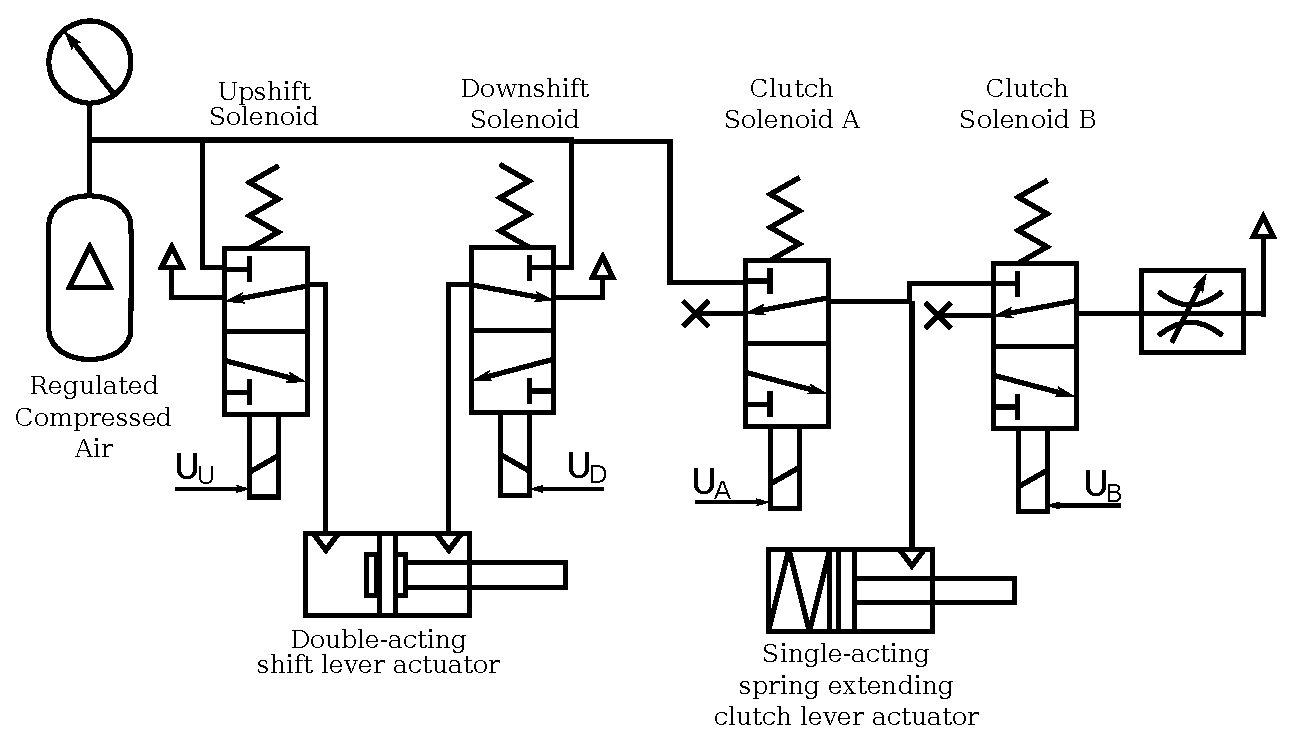
\includegraphics[scale=0.5]{design/figures/pneumatics}
	\caption{Transmission control pneumatics design.}
	\label{fig:pneumatics_design}
\end{figure}

\subsection{Clutch Lever Actuation}
\nomenclature{PWM}{Pulse Width Modulation}
\nomenclature{$U_U$, $U_D$}{Output signals from the transmission controller to the upshift and downshift solenoids.}
\nomenclature{$U_A$, $U_B$}{Pulse width modulated output signals from the transmission controller to clutch solenoids A and B.}

The three approaches described in \cite{pneumatic_actuator, adaptive_pneumatic, accurate_position} considered the possibility of a highly dynamic load on the actuator. The load seen by the clutch actuator is far more predictable than the loads they expected and is only uni-directional. Since the vehicle is only equipped with a limited supply of air, conservation is a concern. Taking these factors into account, a single-acting cylinder with a return spring is specified for the clutch, and we propose a new valving scheme that allows a degree of controllability over the actuator while conserving as much air as possible.

The cylinder visible on the right of Fig. \ref{fig:pneumatics_design}, actuates the clutch lever. Precise control of the clutch is accomplished with fast solenoid valves \emph{Clutch Solenoid A} and \emph{Clutch Solenoid B}. These valves are signalled with \emph{pulse width modulated} (PWM) signals, which modulate the average mass air flow rate into and out separately of the cylinder. Positional feedback for the clutch cylinder is provided by a combination of an internal magnet on the piston in the cylinder and a magnetic sensing membrane potentiometer.

Both clutch solenoids are shown as 3-way (with exhaust ports) valves in Fig. \ref{fig:pneumatics_design}, but the valves are used in a 2-way configuration with the exhaust ports plugged.  This results in the following operation:

\begin{enumerate}
  \item When the pulse width modulated control signal $U_A$ to Clutch Solenoid A is non-zero, the valve will open, and air will flow into the cylinder at a rate proportional to the duty cycle, disengaging the clutch.
  \item When pulses no longer arrive at Clutch Solenoid A (or the duty cycle of $U_A$ approaches 0), the valve remains closed, and any air in the cylinder is trapped. The clutch maintains is position.
  \item When the pulse width modulated control signal $U_B$ to Clutch Solenoid B is non-zero, the valve will open, and any pressure differential between the cylinder and atmosphere will cause air to flow out of the cylinder to atmosphere at a rate proportional to the duty cycle. The clutch springs and the cylinders' internal spring work to return the actuator position to rest, and the clutch engages.
\end{enumerate}

An additional adjustable flow rate control valve (visible on the far right in Fig. \ref{fig:pneumatics_design}) was added to the design to allow additional tuning for during clutch engagement. The electro-pneumatic actuation system meets the controllability requirements outlined in \ref{sec:goals_transmission} when coupled with the transmission controller on the engine and transmission module. No air is wasted in disengaging the clutch and holding the position because the fill and exhaust operations are separately controlled with two valves.

\subsection{Shift Lever Actuation}

The shift lever does not require the same level of control as the clutch, and as such the design of the valving has not changed over previous implementations. Two binary valves are used with a dual-acting cylinder. The first actuator (visible on the left of Fig. \ref{fig:pneumatics_design}) actuates the shift lever between 3 different positions: up-shift, down-shift, and rest-state. The transmission spring-loads the lever to automatically return to the rest-state, which is half-way through the actuator stroke. Applying pressure to one port will pull the lever up, and applying pressure to the other port will pull the lever down.

Current gear position is determined with a potentiometer that is mechanically linked to the shift drum. Control and timing are generated by the engine and transmission controller.

\section{Engine and Transmission Module}

The engine and transmission module provides optimized selection of the variable-length intake, changes gears at the driver's request without requiring manual clutching, and provides transmission features that make driving easier. Figure \ref{fig:design_engine_overview_block} shows an overview of the engine and transmission module and it's interactions with the environment.

\begin{figure}[H]
	\centering
 	\begin{tikzpicture}[auto, node distance=2cm, draw=black!70, >=stealth', font=\footnotesize]
  \node [block, blue shiny, minimum width=4cm, text width=4cm, right=-1cm, node distance=1.5cm] (module) {Engine and\\Transmission Module};

  \node at ($(module.east)+(1cm,0)$) [block, text width=0.8cm] (ecu) {ECU};

  \node [bus, above of=module, node distance=1cm] (bus1) {};
  \node [bus, above of=ecu, node distance=1cm] (bus2) {};

  \draw [<->, thick] (ecu) to (module);

  \draw [-, line width=3pt] (bus1) --  ++(-1cm,0);
  \draw [-, line width=3pt] (bus1) -- node[label=above:CAN Bus]{} (bus2) -- ++(1cm, 0);
  \draw [<->, thick] (module) -- (bus1);
  \draw [<->, thick] (ecu) -- (bus2);

  \node at ($(module.west)!0.5!(module.south)+(0,-1.25cm)$) [red shiny, circle, label={[text width=1.5cm, rotate=90, below=5pt, left=10pt]below right:Servo}] (motor) {M};
  \node [block, left of=motor, node distance=1.5cm, text width=1cm] (intake) {Intake};

  \draw [<-, thick] (intake) -- (motor);
  \draw [<-, thick] (motor) -- ($(module.south west)!(motor.north)!(module.south)$);

  \node [block, below of=module, inner xsep=0pt, right=0cm, node distance=1.5cm] (pneumatics) {Electro-Pneumatic system};
  \draw [<-, thick] (pneumatics) -- ($(module.south west)!(pneumatics.north)!(module.south)$);

  \node [block, right of=pneumatics, text width=2cm, node distance=3cm, above=0.25cm] (shift) {Shift Lever};
  \node [block, right of=pneumatics, text width=2cm, node distance=3cm, below=0.25cm] (clutch) {Clutch Lever};

  \draw [<-, thick, dashed] (clutch) -- ($(pneumatics.north east)!(clutch.west)!(pneumatics.south east)$);
  \draw [<-, thick, dashed] (shift) -- ($(pneumatics.north east)!(shift.west)!(pneumatics.south east)$);

  %%% Legend

  \draw [->, thick] ($(shift.east)+(2cm,0cm)$) -- ++(0.5cm,0) node [label={[font=\tiny]below:Electrical}] {} -- ++(0.5cm,0);
  \draw [->, thick, dashed] ($(clutch.east)+(2cm,0cm)$) -- ++(0.5cm,0) node [label={[font=\tiny]below:Mechanical}] {} -- ++ (0.5cm,0);
\end{tikzpicture}

	\caption{An overview of the engine and transmission module and it's environmental interactions.}
	\label{fig:design_engine_overview_block}
\end{figure}

The intake runner position is mechanically actuated with a \emph{servo motor}. The module generates the control signals required by electro-pneumatic system to actuate both the clutch and shift levers. The ECU interfaces with the module both directly through discrete inputs and through the CAN bus.

\subsection{Driver-Initiated Processes}

The major processes of the engine and transmission module are \emph{up-shifting}, \emph{down-shifting}, and \emph{neutral find}. They are described at a high level using flow charts. Requests to perform these processes are broadcast over the network from the driver interface. The module listens for these requests and executes the correct process accordingly.

\subsubsection{Up-Shifting}

The up-shift procedure is illustrated in \ref{fig:transmission_upshift_flow}. Up-shifting does not require disengaging the clutch, merely a small decrease in engine RPM. The ECU provides a shift-cut feature to cut spark to the engine during a shift operation to avoid the driver having to manually modulate the throttle during a shift.

\begin{figure}[H]
	\centering
	\begin{tikzpicture}[auto, node distance=2cm, draw=black!70, >=stealth', font=\scriptsize]
  \node[start, text width=1.2cm] (start) {Upshift Request};
  \node [decision, right of=start, text width=1cm, inner sep=0pt, node distance=2.5cm] (at_top) {Top\\gear?};
  \node [end, below of=at_top] (done) {Done};
  \node [block, right of=at_top, text width=1.5cm, node distance=2.5cm] (shiftcut) {Enable shiftcut};

  \node [block, right of=shiftcut, text width=1.5cm, node distance=2.5cm] (wait_shiftcut) {Wait for RPM drop below $RPM^{TH}_{cut}$};
  \node [block, right of=wait_shiftcut, text width=1.5cm, node distance=2.5cm] (upshift) {Engage upshift solenoid};
  \node [block, right of=upshift, text width=1.5cm, node distance=2.5cm] (wait_upshift) {Wait for shift feedback};
  \node [block, below of=wait_upshift, text width=1.5cm] (upshift_off) {Disengage upshift solenoid};
  \node [block, left of=upshift_off, text width=1.5cm, node distance=2.5cm] (shiftcut_off) {Disable shiftcut};

  \draw [->, thick] (start) -- (at_top);
  \draw [->, thick] (at_top) -- node[]{yes} (done);
  \draw [->, thick] (at_top) -- node[]{no} (shiftcut);

  \draw [->, thick] (shiftcut) -- (wait_shiftcut);
  \draw [->, thick] (wait_shiftcut) -- (upshift);
  \draw [->, thick] (upshift) -- (wait_upshift);
  \draw [->, thick] (wait_upshift) -- (upshift_off);
  \draw [->, thick] (upshift_off) -- (shiftcut_off);
  \draw [->, thick] (shiftcut_off) -- (done);
\end{tikzpicture}

	\caption{The transmission up-shift procedure.}
	\label{fig:transmission_upshift_flow}
\end{figure}

The up-shift process depends upon engine RPM and gear position, both of which are provided by the ECU. The shift-cut feature is engaged on the ECU to drop the engine RPM by a small amount known as the cut RPM threshold, or $RPM^{TH}_{cut}$. The exact value of $RPM^{TH}_{cut}$ can be tuned on the ECU. Once the RPM reaches the cut threshold, the upshift solenoid is engaged, which actuates the pneumatics to push the shift lever. Once the module receives notification that the current gear has incremented, the pneumatics are relaxed, and shift cut feature is disengaged.

\nomenclature{$RPM^{TH}_{cut}$}{The threshold RPM is expected to drop when shift-cut is engaged for no-lift up-shifting.}

\subsubsection{Down-Shifting}

The down-shift procedure is illustrated in \ref{fig:transmission_downshift_flow}. The downshift procedure differs from the upshift procedure in that the downshift requires use of the clutch. 

\begin{figure}[H]
	\centering
	\begin{tikzpicture}[auto, node distance=2cm, draw=black!70, >=stealth', font=\scriptsize]
  \node[start, text width=1.4cm] (start) {Downshift Request};
  \node [decision, right of=start, text width=1cm, inner sep=0pt, node distance=2.5cm] (in_neutral) {In neutral?};
  \node [end, below of=in_neutral] (done) {Done};
  \node [block, right of=in_neutral, text width=1.5cm, node distance=2.5cm] (clutchin) {Disengage clutch};

  \node [block, right of=clutchin, text width=1.5cm, node distance=2.5cm] (downshift) {Engage downshift solenoid};
  \node [block, right of=downshift, text width=1.5cm, node distance=2.5cm] (wait_downshift) {Wait for shift feedback};
  \node [block, right of=wait_downshift, text width=1.5cm, node distance=2.5cm] (downshift_off) {Disengage downshift solenoid};
  \node [block, below of=downshift_off, text width=1.5cm] (wait_clutchin) {Wait for clutch-in request};
  \node [block, left of=wait_clutchin, text width=1.5cm, node distance=2.5cm] (clutchout) {Engage clutch};

  \draw [->, thick] (start) -- (in_neutral);
  \draw [->, thick] (in_neutral) -- node[]{yes} (done);
  \draw [->, thick] (in_neutral) -- node[]{no} (clutchin);

  \draw [->, thick] (clutchin) -- (downshift);
  \draw [->, thick] (downshift) -- (wait_downshift);
  \draw [->, thick] (wait_downshift) -- (downshift_off);
  \draw [->, thick] (downshift_off) -- (wait_clutchin);
  \draw [->, thick] (wait_clutchin) -- (clutchout);

  \draw [->, thick] (clutchout) -- (done);
\end{tikzpicture}

	\caption{The transmission down-shift procedure.}
	\label{fig:transmission_downshift_flow}
\end{figure}

From the drivers perspective, down-shifting is a two-stage process:

\begin{enumerate}
  \item The driver pulls and holds the down-shift paddle on the steering wheel to request the gear change; and
  \item The driver releases the down-shift paddle to requests the clutch re-engage.
\end{enumerate}

Adding this extra clutch engagement request allows the driver to delay re-engagement of the clutch so that they can blip the throttle to avoid engine compression and the possibility of a spinout when the clutch plates re-engage\footnote{"Blipping" was previously described in Sec. \ref{sec:background_transmission}.}. 

Once the driver requests a down-shift, the clutch is disengaged and the down-shift solenoid is engaged to change gears. Once the correct gear has engaged, the solenoid is disengaged and the controller waits for the driver to release the down-shift paddle. When the paddle is released, the clutch is re-engaged. A minimum clutch disengagement time $t_{clutch_{min}}$ is observed in the event the driver pulls the paddle and releases it without any delay. This parameter is tunable.

\nomenclature{$t^{clutch}_{min}$}{Minimum clutch disengagement time during a downshift request.}

\subsubsection{Neutral Find}

Neutral find can be used by the driver to quickly shift into neutral when entering the pit area, without having to manually cycle through gears. The procedure is illustrated in \ref{fig:transmission_neutralfind_flow}.

\begin{figure}[H]
	\centering
	\begin{tikzpicture}[auto, node distance=2cm, draw=black!70, >=stealth', font=\scriptsize]
  \node[start, text width=1.4cm] (start) {Start};
  \node [decision, right of=start, text width=1.2cm, inner sep=0pt, node distance=2.5cm] (in_neutral1) {Neutral?};
  \node [end, below of=start, node distance=1.5cm] (done) {Done};
  \node [block, right of=in_neutral1, text width=1.5cm, node distance=2.5cm] (clutchin) {Disengage clutch};
  \node [block, right of=clutchin, text width=1.5cm, node distance=2.5cm] (downshift) {Downshift};
  \node [decision, right of=downshift, text width=1.2cm, inner sep=0pt, node distance=2.5cm] (in_neutral2) {Neutral?};

  \node [block, below of=clutchin, text width=1.5cm, node distance=1.5cm] (clutchout) {Engage clutch};

  \draw [->, thick] (in_neutral1.south) -- node[]{yes} (in_neutral1.south |- clutchout);

  \draw [->, thick] (start) -- (in_neutral1);
  \draw [->, thick] (in_neutral1) -- node[]{no} (clutchin);
  \draw [->, thick] (clutchin) -- node[coordinate](x1){} (downshift);
  \draw [->, thick] (downshift) -- (in_neutral2);
  \draw [->, thick] (in_neutral2.north) -- node[above=3pt]{no} ++(0,0.25cm) -| (x1);

  \draw [->, thick] (in_neutral2.south) |- node[]{yes} (clutchout);
  \draw [->, thick] (clutchout) -- (done);
\end{tikzpicture}

	\caption{The transmission neutral find procedure.}
	\label{fig:transmission_neutralfind_flow}
\end{figure}

When the driver engages the neutral find feature, the transmission controller disengages the clutch and downshifts until the neutral sensor indicates the transmission has reached the neutral gear. The clutch lever is then released with the transmission in neutral. If the driver attempts to engage the feature while the vehicle is already in neutral, the procedure is aborted.

\subsection{Variable Intake}

The length of the intake runners is modulated automatically to provide the optimal torque output for the current engine RPM. The control flow chart is shown in Fig. \ref{fig:engine_varintake_flow}. 
\begin{figure}[H]
	\centering
	\begin{tikzpicture}[auto, node distance=2cm, draw=black!70, >=stealth', font=\scriptsize]
  \node [start, text width=1.4cm] (start) {Start};
  \node [block, right of=start, text width=1.5cm, node distance=2.5cm] (update) {Update RPM};
  \node [decision, right of=update, text width=1cm, inner sep=0pt, node distance=2.5cm] (ideal) {Ideal length?};

  \node [block, right of=ideal, text width=1.5cm, node distance=2.5cm] (switch) {Switch lengths};
  \node [block, right of=switch, text width=1.5cm, node distance=2.5cm] (wait) {Wait for lockout};

  \draw [->, thick] (start) -- (update);
  \draw [->, thick] (update) -- (ideal);
  \draw [->, thick] (ideal) -- node[above]{no} (switch);
  \draw [->, thick] (switch) -- (wait);
  \draw [->, thick] (wait) -- ++(0, -1.5cm) node[coordinate](x1){} -| ($(start.east)!0.5!(update.west)$);
  \draw [->, thick] (ideal) -- node[]{yes} (ideal.south |- x1);

\end{tikzpicture}
	\caption{The variable intake adjustment flow.}
	\label{fig:engine_varintake_flow}
\end{figure}

Optimizing the runner length requires coordination with the ECU to acquire the latest RPM values. A set-point RPM value to be determined will act as a cross-over point at which the runner length changes. As the engine RPM crosses over this line, the runner length is modulated. A brief timeout period exists to prevent the runner length from oscillating if the driver is operating near the cross-over point.

\subsection{Advanced Transmission Features}

The transmission portion of the module implements several features to aide the driver. The driver can enable or disable these features from the driver interface. The module will listen for feature requests over the network and act accordingly.

\subsubsection{Auto Up-shift}

This feature of the engine module is aimed primarily at improving performance in the acceleration event. Based on known torque curves, a table of optimal shift points in the RPM range is developed. As the engine reaches the top RPM for a given gear, the engine module will automatically upshift to the next gear, without any driver input. All the driver needs to do is maintain full throttle, and hang on.

\subsubsection{Launch}

Full-throttle launch uses an important feature of the ECU called launch control. From a stand-still, the slip ratio of the driven wheels to the non-driven wheels is monitored, and the engine output power is reduced until the ratio reaches 1:1. Drivers use this feature by maintaining full-throttle at the starting line while holding the brake pedal. As soon as the brake pedal is released, the the engine module will release the clutch in a controlled manner in an attempt to get the best possible acceleration.

\subsubsection{Crawl}

Part-throttle launch is a feature designed to mimic an automatic transmission. By controlling the clutch position, and thereby modulating the amount of torque transferred to the wheels for a short period of time, the car can be made to creep slowly from a stand-still. This will be used when driving up to the starting line of various dynamic events.

\subsection{Hardware}

A high-level overview of the module's hardware design is shown in figure \ref{fig:engine_hardware_design_block}. The module makes use of a \emph{micro-controller} to execute all of the controller software. 

\vspace{1em}
\begin{figure}[H]
	\centering
	\begin{tikzpicture}[auto, node distance=2cm, draw=black!70, >=stealth']

  \node [block, font=\scriptsize, text width=1.5cm, inner xsep=0, minimum height=1cm] (intake) {Intake};
  \node [red shiny, circle, below of=intake, node distance=1.15cm, inner sep=1pt, label=right:Servo] (servo) {M};

  \draw [->, dashed, thick] (servo) -- (intake);

  %%% Balance bar and EOT switches
  \node [block, right of=intake, font=\scriptsize, text width=1.5cm, node distance=3cm, inner xsep=0, minimum height=1cm] (clutch) {Clutch Actuator};
  \node [block, right of=clutch, font=\scriptsize, text width=1.35cm, inner xsep=0, minimum height=1cm] (clutch_solenoids) {Clutch Solenoids};
  \node [block, right of=clutch_solenoids, font=\scriptsize, text width=1.35cm, inner xsep=0, minimum height=1cm] (shift_solenoids) {Shift Solenoids};
  \node [block, right of=shift_solenoids, font=\scriptsize, text width=1.5cm, inner xsep=0, minimum height=1cm] (shifter) {Shift Actuator};

  \node at ($(clutch_solenoids)!0.5!(shift_solenoids)+(0,-2cm)$)
    [block, node distance=1cm, text width=2.5cm, font=\scriptsize, minimum width=3cm] (driver) {Solenoid Drivers};

  \node [block, right of=shifter, font=\scriptsize, text width=1.5cm, inner xsep=0, minimum height=1cm, node distance=3cm] (ecu) {ECU};

  \draw [<-, thick] (clutch_solenoids) -- ($(driver.north west)!(clutch_solenoids.south)!(driver.north east)$);
  \draw [<-, thick] (shift_solenoids) -- ($(driver.north west)!(shift_solenoids.south)!(driver.north east)$);
  \draw [->, dashed, thick] (clutch_solenoids) to (clutch);
  \draw [->, dashed, thick] (shift_solenoids) to (shifter);

  \draw [->, thick] (shifter) to (ecu);

  \node [block, below of=clutch, text width=1.5cm] (adc) {ADC};
  \draw [->, thick] (clutch) to (adc);

  %%% Microcontroller block
  \path ($(intake.south west |- adc.south west) + (0,-1cm)$) node (mu1) {};
  \path ($(shifter.south east |- driver.south east) + (0,-1cm)$) node (mu2) {};

  \node [block, fit=(mu1) (mu2), inner xsep=0, minimum height=1cm] (micro) {Microcontroller};

   \draw [<-, thick] (servo.south) -- ($(micro.north west)!(servo.south)!(micro.north east)$);
   \draw [->, thick] (adc.south) -- ($(micro.north west)!(adc.south)!(micro.north east)$);
   \draw [<-, thick] (driver.south) -- ($(micro.north west)!(driver.south)!(micro.north east)$);

% 
%   \draw [->, thick] (eot1.south) -- ($(micro.north west)!(eot1.south)!(micro.north east)$);
%   \draw [->, thick] (eot2.south) -- ($(micro.north west)!(eot2.south)!(micro.north east)$);
% 
%   \draw [<-, thick] (driver.south) -- ($(micro.north west)!(driver.south)!(micro.north east)$);

  \draw [<-, thick] (ecu.south) |- ($(shifter.south) + (0,-0.5cm)$) node[name=t]{} -- ($(micro.north west)!(t)!(micro.north east)$);

  %%% CAN Bus

  \node at ($(micro.east)+(1.5cm,0)$) [block, name=can, inner xsep=2pt] {CAN Transceiver};
  \draw [<->, thick] (micro) to (can);
  \draw [-, line width=3pt] (ecu.east) -- ++(0.5cm,0) |- node[name=can1,coordinate,label={[rotate=90]below:CAN Bus}]{} (can);
  \draw [-, line width=3pt] (can1) -- ++(0,-1cm);

  %%% Background

   \begin{pgfonlayer}{background}
     \path (intake.south west |- adc.north west)+(-0.3,0.3) node (a) {};
     \path (can.south east)+(+0.2,-0.2) node (b) {};
     \path[module] (a) rectangle (b);
   \end{pgfonlayer}

  %%% Legend

  \draw [->, thick] ($(micro.south west)+(0.5cm,-0.5cm)$) -- ++(0.5cm,0) node [label={[font=\tiny]below:Electrical}] {} -- ++(0.5cm,0);
  \draw [->, thick, dashed] ($(micro.south west)+(2cm,-0.5cm)$) -- ++(0.5cm,0) node [label={[font=\tiny]below:Mechanical}] {} -- ++ (0.5cm,0);
\end{tikzpicture}

	\caption{A block diagram of the engine and transmission module hardware.}
	\label{fig:engine_hardware_design_block}
\end{figure}

\nomenclature{ADC}{Analog-to-Digital Converter}
\nomenclature{GPIO}{General Purpose Input-Output}

Inter-module communication over the CAN bus is mediated with a \emph{CAN transceiver}. An \emph{analog-to-digital converter} (ADC) samples the position of the clutch. Unique to the module are high-current \emph{solenoid driver} that are used to engage the solenoid valves that actuate the clutch and shift levers. Discrete signals to the ECU are connected to \emph{general purpose input-output} (GPIO) lines of the micro-controller.

\subsubsection{Micro-controller}

\nomenclature{EEPROM}{Electronically-Erasable Programmable Read-Only Memory}

The main purpose of the micro-controller is to execute system control software. The micro-controller should be in-circuit programmable and debuggable to speed development, with a built-in CAN controller. It should also have built-in \emph{electronically-erasable programmable read-only memory} (EEPROM) for holding configuration parameters.

\subsubsection{CAN Transceiver}

The CAN transceiver translates the digital bits generated by the CAN controller into a differential line-coded signal suitable for broadcasting over the bus. Both ends of a CAN bus must be terminated with a \unit{120}{\ohm} resistor \cite{MCP2551}. The module should be configurable to terminate the bus if desired.

\subsubsection{Analogue-to-Digital Converters}

The analogue-to-digital converters sample the clutch position sensor. The output voltage of the particular sensor used is \unit{0-5}{\volt}, corresponding to 0-100\% engagement of the clutch. The required sampling frequency is \unit{1}{\kilo\hertz}.

\subsubsection{Solenoid Drivers}

High-current solenoid drivers provide current to the solenoids that actuate the clutch and shift levers. The actual amount of current required depends on the particular implementation. We must use drivers that can source enough current to provide the torque required to actuate the clutch and shift levers. 
 
\subsubsection{ECU Control Signals}

The engine and transmission module have several outputs to control pins on the ECU:

\begin{itemize}
  \item the launch control pin, which enables and disables the launch control feature;
  \item the shift cut pin, which, when held high, enables shift cut;
  \item the traction cut percent pin, which is a \unit{0-5}{\volt} analog input that sets the amount of wheel slip threshold for traction control;
  \item the traction control on/off pin, which toggles the traction control feature; and
  \item the traction control wet/dry pin, which swaps between two traction control presets.
\end{itemize}

\subsection{Software}

A block-diagram overview of the software design is shown in Fig. \ref{fig:engine_software_design_block}. The functionality of the system is separated into an \emph{intake manager} and a \emph{transmission manager}. The managers interact with a set of \emph{hardware abstraction interfaces} to perform their tasks. A \emph{PWM generator} provides the signals required to interact with the electro-pneumatic system. The entire process is overseen by a \emph{module coordinator}.

\begin{figure}[H]
	\centering
%	\tikzstyle{big arrow} = [>=latex, line width=4pt, gray]

\begin{tikzpicture}[auto, node distance=2cm, draw=black!70, >=stealth', font=\scriptsize]
  %\draw[help lines] (-1,-5) grid (8,2);
  
  \node [block, minimum width=2cm, inner xsep=0] (servo) {Servo Interface};

  \node [block, grey shiny, minimum width=5cm, inner xsep=0, right of=servo, right=-1cm, text width=5cm, node distance=3cm] (intake_manager) {Intake Manager};

  \node [block, minimum width=2cm, inner xsep=0, below of=intake_manager, node distance=2cm, right=-2.5cm, minimum height=1cm] (can) {CAN Interface};
  \node [block, minimum width=2cm, inner xsep=0, below of=intake_manager, node distance=2cm, left=-2.5cm, minimum height=1cm] (nv) {NV Storage Interface};

  \node [block, grey shiny, minimum width=5cm, inner xsep=0, below of=intake_manager, text width=5cm, node distance=4cm] (transmission_manager) {Transmission Manager};

  \node [block, minimum width=2cm, inner xsep=0, below of=servo, node distance=4cm] (pwm) {PWM Generator};

  \node [block, minimum width=2cm, inner xsep=0, below of=transmission_manager, node distance=1.5cm, right=-2.5cm, minimum height=1cm] (adc) {ADC Interface};
  \node [block, minimum width=2cm, inner xsep=0, below of=transmission_manager, node distance=1.5cm, left=-2.5cm, text width=1.5cm, minimum height=1cm] (gpio) {GPIO Interface};

  \node [block, minimum width=2cm, inner xsep=0, right of=nv, node distance=3cm] (coordinator) {Module Coordinator};
  \node [block, minimum width=2cm, inner xsep=0, right of=coordinator, node distance=3cm] (scheduler) {Event Scheduler};

  \draw [<-, big arrow] (servo) -- (intake_manager);
  \draw [<-, big arrow] (pwm) -- (transmission_manager);

  \draw [<->, big arrow] (can.north) -- ($(intake_manager.south west)!(can.north)!(intake_manager.south east)$);
  \draw [<->, big arrow] (nv.north) -- ($(intake_manager.south west)!(nv.north)!(intake_manager.south east)$);

  \draw [<->, big arrow] (can.south) -- ($(transmission_manager.north west)!(can.south)!(transmission_manager.north east)$);
  \draw [<->, big arrow] (nv.south) -- ($(transmission_manager.north west)!(nv.south)!(transmission_manager.north east)$);

  \draw [<-, big arrow] (adc.north) -- ($(transmission_manager.south west)!(adc.north)!(transmission_manager.south east)$);
  \draw [->, big arrow] (gpio.north) -- ($(transmission_manager.south west)!(gpio.north)!(transmission_manager.south east)$);

  \draw [<->, big arrow] (transmission_manager) -| node[](x1){} (coordinator);
  \draw [->, big arrow] (x1) -| (scheduler);
  \draw [<->, big arrow] (coordinator) -- (scheduler);

  \draw [<->, big arrow] (intake_manager) -| (coordinator);
 
\end{tikzpicture}

	\caption{The engine and transmission module software block diagram.}
	\label{fig:engine_software_design_block}
\end{figure}

\subsubsection{Hardware Abstraction Interfaces}

The external hardware and micro-controller features that are needed by the intake and pressure managers are best abstracted through \emph{hardware abstraction interfaces}. This allows for a modular design that is not intimately mated with any particular external hardware choice. 

Abstraction interfaces required by the engine and transmission module include a \emph{CAN interface}, \emph{servo interface}, a \emph{general-purpose input-output (GPIO) interface}, an \emph{analog-to-digital (ADC) interface} and a \emph{non-volatile storage interface}. A summary of the purpose for each interface is listed below.

\begin{itemize}

\item The CAN interface, common to each module, enables network communication over the CAN bus. Managers can schedule packets for transmission, and incoming packets can be routed to the appropriate manager.

\item The solenoid driver interface converts the logic-level on-off commands to control signals for the high-current solenoid driver.

\item The servo interface takes a positional adjustment command from the program and utilizes the pulse-width generator to generate a drive signal for the servo motor with the correct duty cycle and frequency.

\item The GPIO interface provides a means of setting any of the control lines connected to the ECU. It is responsible for generating the correct logic levels for a given ECU feature request.

\item The analog-to-digital (ADC) interface communicates with the hardware analog-to-digital converter. It can initiate a sampling cycle on either return the results to the program for further processing.

\item The non-volatile storage interface can read and write data to and from \emph{non-volatile random-access memory} (NVRAM). This enables configuration parameters to be stored and read even if the module loses power or is reset.

\end{itemize}

\subsubsection{Event Scheduler}

The event scheduler allows for complex sequencing of events in time. It allows for new events to be scheduled at some point in the future.
The scheduler will continuously update the schedule and signal the module coordinator to execute events that are now current. The scheduler requires a resolution of \emph{1}{\milli\second} to be useful to the transmission manager for scheduling solenoid actuation events.

\subsubsection{PWM Generator}

The PWM generator generates the signals required by the transmission manager to engage the clutch lever solenoids. To meet the goals of the transmission system, the signals must have a frequency of at least \unit{20}{\hertz} and a 1\% duty cycle resolution. Since there are two solenoids to be activated, the generator must be able to offer two independent output channels.

\subsubsection{Transmission Manager}

The transmission manager listens to shifting and feature requests from the driver over the network. It implements the up-shift, down-shift, and neutral find processes. It is also responsible for implementing the advanced transmission features such as launch and crawl.

The transmission manager uses the event scheduler to sequence the complex series of actuation vectors required by up-shifting and down-shifting. It also implements the feedback control system required by the electro-pneumatic system to smoothly actuate the clutch lever. Timing signals are generated with the help of the PWM generator.

\subsubsection{Intake Manager}

The intake manager continuously monitors the engine RPM being broadcast by the ECU. It adjusts the intake runner length based on a cross-over point determined by dynometer testing. Adjustments to the runner length are made via the servo interface.


\subsubsection{Module Coordinator}

Each of the processes implemented by the managers are made up of several states. Asynchronous events, such as a request to change gears, are handled by the managers themselves. The module coordinator contains the low-level state machine mechanisms needed by the two managers to transition between their internal states. It keeps track of the current state of the system, and also initializes all of the hardware abstraction interfaces and managers at start-up time. The coordinator also interacts with the event scheduler, waiting for pending events to be executed and then executing them.

\section{Braking Module\label{sec:Braking-Module-Design}}

The braking module adjusts the brake bias electronically as requested by the driver. It also provides the ability to calibrate itself to account for mechanical wear and to account for a degree of component tolerance that may cause unwanted rotation of the balance bar. Figure \ref{fig:design_brake_overview_block} shows an overview of the braking module and its interactions with the environment. 

\begin{figure}[H]
\centering
\begin{tikzpicture}[auto, node distance=2cm, draw=black!70, >=stealth', font=\footnotesize]
  \node [block, minimum width=2cm, inner xsep=0] (pressure1) {Front Pressure Sensor};
  \node [block, minimum width=2cm, inner xsep=0, right of=pressure1, node distance=4cm] (pressure2) {Front Pressure Sensor};

  \node [block, blue shiny, minimum width=6cm, text width=4cm, below of=pressure1, right=-1cm, node distance=1.5cm] (module) {Braking Module};

  \node [block, below of=pressure1, right=-1cm, node distance=3cm, text width=1.1cm] (eot1) {Left EOT Switch};
  \node [block, below of=pressure2, left=-1cm, node distance=3cm, text width=1.1cm] (eot2) {Right EOT Switch};

  \node at ($(eot1)!0.5!(eot2)$) [red shiny, circle, label={[text width=1.5cm, rotate=90, below=5pt, left=10pt]below right:Stepper Motor}] (motor) {M};

  \node [rectangle, below of=motor, minimum width=2cm, label=below:Bias Bar, pattern=north east lines, node distance=1cm] (bias) {};

  \draw [->, thick] (pressure1.south) to ($(module.north west)!(pressure1.south)!(module.north east)$);
  \draw [->, thick] (pressure2.south) to ($(module.north west)!(pressure2.south)!(module.north east)$);

  \draw [->, thick] (eot1.north) to ($(module.south west)!(eot1.north)!(module.south east)$);
  \draw [->, thick] (eot2.north) to ($(module.south west)!(eot2.north)!(module.south east)$);

  \draw [<-, thick] (motor.north) to ($(module.south west)!(motor.north)!(module.south east)$);
  \draw [->, thick, dashed] (motor.south) to ($(bias.north west)!(motor.south)!(bias.north east)$);

  \draw [->, thick, dashed] (bias) -| (eot1);
  \draw [->, thick, dashed] (bias) -| (eot2);

  %%% CAN Bus

  \node [bus, name=can1, right of=module, label={[rotate=90, left=0.75cm]below right:CAN Bus}, node distance=3.5cm] {CAN Bus};
  \node [bus, name=can2, below of=can1, node distance=1cm] {};
  \node [bus, name=can3, above of=can1, node distance=1cm] {};

  \draw [<->, thick] (module) to (can1);
  \draw [-, line width=3pt] (can1) -- (can2);
  \draw [-, line width=3pt] (can1) -- (can3);

  %%% Legend

  \draw [->, thick] ($(eot2.east)+(2cm,0cm)$) -- ++(0.5cm,0) node [label={[font=\tiny]below:Electrical}] {} -- ++(0.5cm,0);
  \draw [->, thick, dashed] ($(eot2.south east)+(2cm,0cm)$) -- ++(0.5cm,0) node [label={[font=\tiny]below:Mechanical}] {} -- ++ (0.5cm,0);
\end{tikzpicture}
\caption{Overview of the braking module and it's environment.}
\label{fig:design_brake_overview_block}
\end{figure}

\nomenclature{EOT}{End of Travel}
A \emph{stepper motor} is connected to the balance bar and used to rotate it to the desired position. The motor should be bi-directional. Two \emph{end-of-travel} (EOT) switches are used to determine when the balance bar is at its end of travel. \emph{Pressure sensors} on the front and rear braking cylinders are used to determine the current pressure in each system. These components were chosen as part of the mechanical design of the brake pedal assembly by another team member. The actual choice of stepper motor has yet to be determined.

\subsection{Driver-Initiated Processes \label{sec:braking_processes}}

The major processes of the braking module are \emph{brake bias adjustment}, \emph{brake bias calibration}, and \emph{pressure calibration}. Requests to perform either of the processes are broadcast over the network from the driver interface. The module listens for these requests and executes the correct process accordingly. 

\subsubsection{Brake Bias Adjustment}

The brake bias adjustment procedure is shown in Fig. \ref{fig:design-braking-bias-adjustment}. The module performs a series of safety checks before rotating the balance bar to adjust the relative force distribution between the two brake master cylinders.

\begin{figure}[H]
	\centering
	\begin{tikzpicture}[auto, node distance=2cm, draw=black!70, >=stealth', font=\scriptsize]
  \node [start] (start) {Start};
  \node [decision, right of=start, text width=1cm, inner sep=0pt] (valid_bias) {Valid Bias?};
  \node [end, below of=start, node distance=1cm] (abort) {Abort};

  \node [block, right of=valid_bias, text width=1.5cm, inner xsep=0pt, node distance=2.5cm] (calc) {Calculate Offset Steps};
  \node [block, right of=calc, text width=1.5cm, inner xsep=0pt, node distance=2.5cm] (step) {Step by offset};
  \node [block, right of=step, text width=1cm, inner xsep=0pt] (store) {Store new offset};
  \node [end, right of=store] (done) {Done};

  \draw [->, thick] (start) to (valid_bias);
  \draw [->, thick] (valid_bias.south) |- node[below]{no} (abort);
  \draw [->, thick] (valid_bias) to node[above]{yes} (calc);
  \draw [->, thick] (calc) to (step);
  \draw [->, thick] (step) to (store);
  \draw [->, thick] (store) to (done);
\end{tikzpicture}

	\caption{Flow-chart for the brake bias adjustment procedure.}
	\label{fig:design-braking-bias-adjustment}
\end{figure}

Of prime importance is that the vehicle is not in motion and the brakes are not engaged while the adjustment is underway. The desired bias ratio is also validated before any adjustment is attempted. If the vehicle is stopped, the brakes are not engaged, and the request is valid, the adjustment may proceed. The module calculates the number of steps required to move from the current position to the desired offset and signals the motor to advance this many steps in the correct direction.

\subsubsection{Brake Bias Calibration}

A flow-chart of the brake bias calibration procedure is shown in Fig. \ref{fig:brake_bias_calibration_flow}. By recording the number of steps it takes to rotate the balance bar from through its range of motion, we can determine the correct centre point for the bias bar. 

\begin{figure}[H]
	\centering
	\begin{tikzpicture}[auto, node distance=2cm, draw=black!70, >=stealth', font=\scriptsize]
  \node [start] (start) {Start};

  \node [block, right of=start, text width=1cm, inner xsep=0pt] (step_left) {Step Left};
  \node [decision, right of=step_left, text width=1.0cm, inner sep=0pt] (at_left) {At leftend?};

  \node [block, right of=at_left, text width=1cm, inner xsep=0pt] (step_right) {Step Right};
  \node [block, right of=step_right, text width=1cm, inner xsep=2pt] (count) {Add to count};
  \node [decision, right of=count, text width=1cm, inner sep=0pt] (at_right) {At rightend?};

  \node [block, below of=at_right, text width=2cm, inner xsep=2pt, node distance=2.5cm] (adjust) {Adjust bias to old value};
  \node [block, left of=adjust, text width=1.5cm, inner xsep=2pt, node distance=3cm] (store) {Store calibration};
  \node [end, left of=store, node distance=7cm] (end) {Done};

  \draw [->, thick] (start) to node[coordinate, name=x1]{} (step_left);
  \draw [->, thick] (step_left) to (at_left);
  \draw [->, thick] (at_left.south) -- ++(0,-0.25) node[below]{no} -| (x1);
  \draw [->, thick] (at_left.east) to node[name=x2]{yes} (step_right);
  \draw [->, thick] (step_right) to (count);
  \draw [->, thick] (count) to (at_right);
  \draw [->, thick] (at_right.south) -- ++(0,-0.25) node[below]{no} -| (x2);

  \draw [->, thick] (at_right.east) -- ++(0.5,0) node[above]{yes} |- (adjust);
  \draw [->, thick] (adjust) to (store);
  \draw [->, thick] (store) to (end);
\end{tikzpicture}

	\caption{Flow-chart for the brake bias calibration procedure.}
	\label{fig:brake_bias_calibration_flow}
\end{figure}

The first step in calibrating the brake bias is to rotate the balance bar to its leftmost point of travel, where it pushes on the left end-of-travel switch. This signals the module that the leftmost extreme has been reached. Next, the balance bar is rotated to its rightmost point of travel, until it pushes on the right end-of-travel switch. The module counts the steps required to travel through its range of motion and saves the count in non-volatile parameter storage. Finally, the brake bias ratio is adjusted back to its previous value.

\subsubsection{Pressure Calibration}

The pressure sensor calibration routine is outlined in Fig. \ref{fig:brake_pressure_calibration_flow}. The module keeps track of the minimum and maximum pressures that will be present in both the front and rear systems. This allows it to determine when the brakes are engaged, and to what extent.

\begin{figure}[H]
	\centering
	\begin{tikzpicture}[auto, node distance=2cm, draw=black!70, >=stealth', font=\scriptsize]
  \node [start] (start) {Start};
  \node [decision, right of=start, right=0cm, text width=1.4cm, inner sep=0pt] (min) {Min Applied?};
  \node [block, right of=min, text width=2cm, inner xsep=0pt, node distance=3cm] (sample1) {Sample Pressures};
  \node [decision, right of=sample1, right=0cm, text width=1.4cm, inner sep=0pt] (max) {Max Applied?};
  \node [block, right of=max, text width=2cm, inner xsep=0pt, node distance=3cm] (sample2) {Sample Pressures};

  \node [decision, below of=sample2, text width=1.4cm, inner sep=0pt, node distance=2.5cm] (valid) {Valid samples?};
  \node [block, left of=valid, text width=1.5cm, inner xsep=2pt, node distance=3cm] (save) {Save Calibration};

  \node [end, below of=save] (success) {Success};
  \node [end, below of=valid] (fail) {Fail};

  \draw [->, thick] (start) -- ($(start.east)!0.5!(min.west)$) node[name=x1,coordinate]{} -- (min);
  \draw [->, thick] (min.south) -- ++(0,-0.25cm) node[below]{no} -| (x1);
  \draw [->, thick] (min) to node [] {yes} (sample1);

  \draw [->, thick] (sample1) to node [name=x2]{} (max);
  \draw [->, thick] (max.south) -- ++(0,-0.25cm) node[below]{no} -| (x2);
  \draw [->, thick] (max) to node [] {yes} (sample2);

  \draw [->, thick] (sample2) to (valid);
  \draw [->, thick] (valid) to node [above] {yes} (save);

  \draw [->, thick] (save) to (success);
  \draw [->, thick] (valid.south) to node [] {no} (fail);

\end{tikzpicture}
	\caption{Flow-chart for the brake pressure calibration sequence.}
	\label{fig:brake_pressure_calibration_flow}
\end{figure}

The first step of pressure calibration is to ask the driver to apply minimum pressure. The brake module signals the driver interface to request the driver take their foot off the brake. Once done, the driver interface signals the brake module that minimum pressure has been applied. The brake module then samples the current pressure in both systems. This procedure is repeated for maximum pressure by asking the driver to push on the brake as hard as possible. If the samples are valid, meaning the minimum pressures are less than the maximum pressures and there is a minimum pressure difference between fully-released and fully-applied, the sampled pressures are stored in non-volatile memory.

\subsection{Hardware}

A high-level overview of the module's hardware design is shown in Fig. \ref{fig:brake_hardware_design_block}. Like the other modules, the heart of the brake module is a micro-controller that runs the software necessary to implement all of the required features. 

\begin{figure}[H]
\centering
\begin{tikzpicture}[auto, node distance=2cm, draw=black!70, >=stealth']
%  \draw[help lines] (-3,-5) grid (8,2);

  %%% Pressure Sensors
  \node [block, name=pressure1, font=\scriptsize, text width=1.5cm, inner xsep=0] {Front Pressure Sensor};
  \node [block, name=pressure2, right of=pressure1, font=\scriptsize, text width=1.5cm, inner xsep=0] {Rear Pressure Sensor};

  %%% Balance bar and EOT switches
  \node [block, name=eot1, right of=pressure2, font=\scriptsize, text width=1.5cm, node distance=3cm] {Left EOT Switch};
  \node [block, name=balance, right of=eot1, font=\scriptsize, text width=1.25cm, inner xsep=0] {Balance Bar};
  \node [block, name=eot2, right of=balance, font=\scriptsize, text width=1.5cm] {Right EOT Switch};

  \node [red shiny, circle, below of=balance, name=motor, node distance=1cm, inner sep=1pt] {M};
  \node [block, below of=motor, node distance=1cm, text width=1.5cm, font=\scriptsize] (driver) {Stepper Driver};

  \draw [->, dashed, thick] (balance) -- (eot1);
  \draw [->, dashed, thick] (balance) -- (eot2);
  \draw [->, dashed, thick] (motor) -- (balance);
  \draw [->, thick] (driver) -- (motor);

  \node [block, name=adc1, below of=pressure1, text width=1.5cm] {ADC};
  \node [block, name=adc2, below of=pressure2, text width=1.5cm] {ADC};

  %%% Microcontroller block
  \path ($(adc1.south west)+(0,-1cm)$) node (mu1) {};
  \path ($(adc1.south west -| eot2.south east) + (0,-1cm)$) node (mu2) {};

  \node [block, name=micro, fit=(mu1) (mu2), inner xsep=0, minimum height=1cm] {Microcontroller};

  \draw [->, thick] (pressure1) to (adc1);
  \draw [->, thick] (pressure2) to (adc2);
  \draw [->, thick] (adc1.south) -- ($(micro.north west)!(adc1.south)!(micro.north east)$);
  \draw [->, thick] (adc2.south) -- ($(micro.north west)!(adc2.south)!(micro.north east)$);

  \draw [->, thick] (eot1.south) -- ($(micro.north west)!(eot1.south)!(micro.north east)$);
  \draw [->, thick] (eot2.south) -- ($(micro.north west)!(eot2.south)!(micro.north east)$);

  \draw [<-, thick] (driver.south) -- ($(micro.north west)!(driver.south)!(micro.north east)$);

  %%% CAN Bus

  \node at ($(micro.east)+(2cm,0)$) [block, name=can, node distance=2cm, inner xsep=2pt] {CAN Transceiver};

  \draw [<->, thick] (micro) to (can);

  \node [bus, name=can1, above of=can, label=above:CAN Bus, node distance=2.5cm] {CAN Bus};
  \node [bus, name=can2, left of=can1, node distance=1cm] {};
  \node [bus, name=can3, right of=can1, node distance=1cm] {};

  \draw [-, line width=3pt] (can) -- (can1);
  \draw [-, line width=3pt] (can1) -- (can2);
  \draw [-, line width=3pt] (can1) -- (can3);

  %%% Background

  \begin{pgfonlayer}{background}
    \path (adc1.north west)+(-0.3,0.3) node (a) {};
    \path (can.south east)+(+0.2,-0.2) node (b) {};
    \path[module] (a) rectangle (b);
  \end{pgfonlayer}

  %%% Legend

  \draw [->, thick] ($(micro.south west)+(0.5cm,-0.5cm)$) -- ++(0.5cm,0) node [label={[font=\tiny]below:Electrical}] {} -- ++(0.5cm,0);
  \draw [->, thick, dashed] ($(micro.south west)+(2cm,-0.5cm)$) -- ++(0.5cm,0) node [label={[font=\tiny]below:Mechanical}] {} -- ++ (0.5cm,0);
\end{tikzpicture}

\caption{Block diagram of the braking module hardware.}
\label{fig:brake_hardware_design_block}
\end{figure}

The module communicates over the bus using a CAN transceiver. A pair of analog-to-digital converters (similar to those used in the engine and transmission module) sample the brake pressure sensors. Unique to the brake module is a \emph{stepper motor driver} that provides the signals necessary to drive the stepper motor connected to the balance bar. The micro-controller interfaces to the end-of-travel switches without any extra hardware.

\subsubsection{Stepper Motor Driver}

The stepper motor driver generates the signals required to drive the stepper motor connected to the balance bar. Approximately \unit{150}{mA} of current are required to generate the torque required to spin the balance bar \footnote{This figure was supplied by the team member responsible for the braking pedal assembly.}.

\subsubsection{Analogue-to-Digital Converters (ADC)}

The ADCs sample the output voltage from pressure sensors attached to the front and rear brake master cylinders. The output voltage of the particular sensors used is \unit{0-5}{\volt}, corresponding to \unit{0-10}{\mega\pascal}. The expected maximum brake pressure is somewhere around \unit{7}{\mega\pascal}. To achieve resolution of \unit{100}{\kilo\pascal}, a 10-bit ADC is sufficient. The pressure values are sampled at \unit{10}{\hertz}.

\subsubsection{End-of-Travel Sensing Switches}

Two end-of-travel switches are tripped whenever the balance bar reaches its leftmost or rightmost extremes. The switches are normally high-impedance, and become switched to ground when they are pushed by a metal tab attached to the balance bar assembly. 

\subsection{Software}

A block-diagram overview of the software design is shown in Fig. \ref{fig:brake_software_design_block}. The functionality of the system is separated into a \emph{bias manager} and a \emph{pressure manager}. Like the engine and transmission module, the managers interact with a set of hardware abstraction interfaces to perform their tasks, and the entire process is overseen by a \emph{module coordinator}.

\begin{figure}[H]
	\centering
	\tikzstyle{big arrow} = [>=latex, line width=4pt, gray]

\begin{tikzpicture}[auto, node distance=2cm, draw=black!70, >=stealth']
  \node [block, minimum width=2cm, inner xsep=0] (stepper) {Stepper Interface};
  \node [block, minimum width=2cm, inner xsep=0, right of=stepper, node distance=3cm] (io) {I/O Interface};

  \node [block, grey shiny, minimum width=5cm, inner xsep=0, below of=stepper, right=-1cm, text width=5cm, node distance=2cm] (bias_manager) {Bias Manager};

  \node [block, minimum width=2cm, inner xsep=0, below of=stepper, node distance=4cm] (can) {CAN Interface};
  \node [block, minimum width=2.2cm, inner xsep=0, below of=io, node distance=4cm] (nv) {NV Storage Interface};
  \node [block, blue shiny, minimum width=2.5cm, text width=2.2cm, inner xsep=0, right of=nv, node distance=3cm] (coordinator) {Module Coordinator};
  \node [block, minimum width=2cm, inner xsep=0, left of=can, node distance=3cm] (adc) {ADC Interface};

  \node [block, grey shiny, minimum width=5cm, inner xsep=0, below of=can, right=-1cm, text width=5cm, node distance=2cm] (pressure_manager) {Pressure Manager};

  \draw [<-, big arrow] (stepper.south) -- ($(bias_manager.north west)!(stepper.south)!(bias_manager.north east)$);
  \draw [->, big arrow] (io.south) -- ($(bias_manager.north west)!(io.south)!(bias_manager.north east)$);

  \draw [<->, big arrow] (can.north) -- ($(bias_manager.south west)!(can.north)!(bias_manager.south east)$);
  \draw [<->, big arrow] (nv.north) -- ($(bias_manager.south west)!(nv.north)!(bias_manager.south east)$);

  \draw [<->, big arrow] (can.south) -- ($(pressure_manager.north west)!(can.south)!(pressure_manager.north east)$);
  \draw [<->, big arrow] (nv.south) -- ($(pressure_manager.north west)!(nv.south)!(pressure_manager.north east)$);

  \draw [<->, big arrow] (bias_manager) -| (coordinator);
  \draw [<->, big arrow] (pressure_manager) -| (coordinator);
  \draw [->, big arrow] (adc) |- (pressure_manager);

  \draw [-, thick] ($(coordinator.south)!0.5!(coordinator.south west)$) |- ($(nv.south)!0.5!(nv.south east)+(0,-0.6cm)$) node [name=x, inner sep=0]{};
  \draw [->, thick] (x) -- ($(nv.south)!0.5!(nv.south east)$);
  \draw [->, thick] (x) -| ($(can.south)!0.5!(can.south east)$);

  \draw [-, thick] (adc.east) -| ($(stepper.south west)+(-0.5cm,-0.6cm)$) node [name=x2, inner sep=0]{};
  \draw [->, thick] (x2) -| ($(stepper.south)!0.5!(stepper.south east)$);
  \draw [->, thick] (x2) -| ($(io.south)!0.5!(io.south east)$);
  
\end{tikzpicture}

	\caption{Block diagram of the braking module software.}
	\label{fig:brake_software_design_block}
\end{figure}

Several hardware abstraction interfaces link the external hardware and micro-controller features to the bias and pressure managers. Unique to the braking module is the \emph{stepper motor interface}. 

\subsubsection{Bias Manager}

The bias manager implements the bias adjustment and bias calibration processes. It listens for requests to initiate either process from the network by way of the CAN interface.

When asked to adjust the brake bias, the bias manager coordinates with the pressure manager to determine if the brakes are being applied, and with the engine and transmission controller to determine if the vehicle is in motion. It performs the calculations required to calculate the new bias position, and adjusts the balance bar accordingly by sending motor step commands to the stepper motor interface.

Bias calibration requires similar coordination to ensure a safe operating state. The bias manager again uses the stepper motor interface to move the balance bar between its extremes. Calibration data is loaded at start-up and stored after calibration in NVRAM by way of the non-volatile storage interface.

\subsubsection{Pressure Manager}

The pressure manager periodically outputs the front and rear brake pressures. It also implements the pressure calibration procedure and listens for calibration requests over the network, similar to the bias manager.

The front and rear pressures are sampled through the ADC interface. The pressure manager uses the CAN interface to output the samples over the network. Current pressure readings are made available to the bias manager to avoid adjusting or calibrating the bias while the brakes are engaged.

The pressure manager communicates with the driver interface through the CAN interface to coordinate the sequence of driver inputs required to calibrate the front and rear brake pressures. Like the pressure manager, calibration data is loaded at start-up and stored after calibration through the non-volatile storage interface.

\subsubsection{Module Coordinator}

Like the module coordinator for the engine and transmission module, the braking module coordinator contains the low-level state machine mechanisms needed by the two managers to transition between their internal states. It keeps track of the current state of the system, and also initializes all of the hardware abstraction interfaces and managers at start-up time. 

\subsubsection{Stepper Motor Interface}

The stepper motor interface takes motor movement commands from the program and converts them into commands for the stepper motor driver. It can direct the stepper motor driver to turn clockwise or counter-clockwise, and move an arbitrary number of steps. 

\subsubsection{GPIO Interface}

The GPIO interface monitors the state of the end-of-travel buttons. It can asynchronously interrupt the program when a change of state occurs. 

\subsubsection{ADC Interface}  

The ADC interface initiates a sampling cycle on either pressure sensor channel. The resulting sample is provided to  the program for further processing. 

\subsubsection{Non-Volatile Storage Interface}

The \emph{non-volatile storage interface} reads and writes calibration data to the non-volatile storage portion of the micro-controller. It is also used to keep track of the current position of the bias bar, so calibration is not required between start-ups.


\section{Telemetry Module\label{sec:Telemetry-Module-Design}}

The \emph{wireless telemetry system} provides a means for multiplexing these data streams and sending them wirelessly to laptops. The vehicle-side of the telemetry system consists of:

\begin{itemize}
\item the \emph{telemetry module}, which gathers and multiplexes the data; and
\item the \emph{wireless modem}, which transmits data wirelessly to a receiver.
\end{itemize}

The remote-side of the telemetry system consists of an off-the-shelf wireless receiver, which receives the data and makes it available on an RS-232 port.


\subsection{Purpose}

Provide a multiplexed virtual serial link between the ECU and the ECU software, and the DAC and the DAC software. Additionally be able to decode the DAC serial data on the car, and inject additional data channels into the DAC serial stream.


\subsection{Processes}


\subsubsection{ECU Transmission Channel}


\subsubsection{DAC Transmission Channel}


\subsubsection{DAC Packet Capture and Injection}


\subsection{Software}


\subsubsection{Wireless Interface Manager }


\subsubsection{Data Multiplexor}


\subsubsection{Data Decoder }


\subsubsection{Packet Injector}


\subsubsection{CAN Interface}


\subsubsection{Main Control Loop}


\subsection{Hardware}


\subsubsection{Microcontroller}


\subsubsection{CAN Transceiver}


\subsubsection{High-Speed UART Bank}


\subsubsection{Wireless Modem}
\section{Driver Interface Module Design\label{sec:Driver-Interface-Module}}


\subsection{Purpose}


\subsection{Processes}


\subsubsection{Driver Controls}
The driver controls consist of three rotary encoder knobs and three buttons. See table \ref{table:driver_controls} for a description of each.

\begin{table}[H]
\caption{Available driver controls.\label{table:driver_controls}}
\centering
\begin{tabular}{|c|c|p{8 cm}|}
	\hline 
	Type & Name & Description \\
	\hline
	\hline 
	Rotary & VDM & Changes the current VDM setting. \\
	\hline 
	Rotary & Option & Changes the currently selected menu option. \\
	\hline
	Rotary & Adjust & Adjusts the value associated with the currently selected menu option. \\
	\hline
	Button & Starter & Engages the automatic start sequence if pressed once, or the manual start sequence if held down.\\
	\hline
	Button & Neutral Find & Activates the neutral-find feature. \\
	\hline
	Button & Diagnostics/Save & Pages through diagnostic information if pressed once, or saves the current dynamic settings to the selected VDM if held down.\\		
	\hline 		
\end{tabular}
\end{table}


\subsubsection{Diagnostic Information}

The interface display panel is a large monochrome \emph{Liquid Crystal Display} (LCD) screen, inset into the steering wheel. The panel provides real-time information to the driver regarding all of the electronic systems in the car. Primary information displayed on the panel includes:

\begin{itemize}
\item the selected gear;
\item the active \emph{vehicle dynamics mode} (VDM);
\item the telemetry signal strength;
\item the engine RPM;
\item the vehicle wheel speed; and
\item the status of the launch control feature.
\end{itemize}

The list of available options and the current value for the selected option is displayed on screen when the driver rotates the option dial. After a timeout period, normal real-time information display resumes. 



\subsubsection{Vehicle Dynamics Mode (VDM)}
\nomenclature{VDM}{Vehicle Dynamics Mode}

The driver interface system provides a method of quickly modifying several dynamic vehicle parameters quickly and easily. For example, an acceleration event calls for launch control, auto-upshift, and a heavy forward brake bias. It is possible to enable all of these features in one step by changing the VDM mode to {}``acceleration''. 

When a new mode is selected, all nodes on the network are notified and synchronized to modify their dynamic parameters in accordance with the specific mode. For example, when the  {}``acceleration'' mode is enabled, the engine module will enable launch control and auto-upshift, and the brake controller will modify the brake bias to a pre-set ratio.

\begin{description}
  \item [{Pit Mode}] enables soft-launch driving characteristics that mimic a fully automatic transmission. This makes slowly driving the car forward from a stand-still far easier, and only requires the driver to take their left foot off the brake, and slightly apply the throttle.
  \item [{Acceleration Mode}] puts the vehicle systems into full-performance characteristics. Launch control is activated. The engine module will watch for a launch signal from the driver, and will automatically up-shift based on the engine RPM.
  \item [{Dynamic Mode}] puts the vehicle systems into a mode that is suitable for the autocross, and the endurance race.
\end{description}


\subsubsection{Parameter Tuning}


\subsection{Software}


\subsubsection{User Interface Manager}


\subsubsection{Driver Control Manager}


\subsubsection{Vehicle Diagnostics Manager}


\subsubsection{Vehicle Dynamic Mode Manager}


\subsubsection{I/O Monitor}


\subsubsection{CAN Interface}


\subsubsection{Main Control Loop}


\subsection{Hardware}


\subsubsection{Microcontroller}


\subsubsection{CAN Transceiver}


\subsubsection{LCD Module}


\subsubsection{Input Knobs and Buttons}


\subsubsection{Paddle Shifters}